\documentclass{article}
\usepackage[margin=1in]{geometry}
\usepackage{booktabs}
\usepackage{enumitem}
\usepackage{xcolor,colortbl}
\usepackage[margin=1in]{geometry} % For better margins
\usepackage{graphicx} % Required for \rotatebox command


\title{Final Assignment}
\author{Ichim Ștefan - Knowledge Discovery using FCA}
\date{\today}

\begin{document}

\maketitle

\section*{Exercise 4: Attribute Exploration: Olympic Sports Analysis}

\subsection*{Domain and Attribute Selection}

The domain chosen for attribute exploration is popular Olympic sports. Ten attributes were selected based on observable characteristics that distinguish different Olympic sports categories.

\textbf{Selected Attributes:}
Team\_Sport, Water\_Based, Indoor\_Venue, Equipment\_Heavy, Contact\_Sport, Timed\_Event, Subjective\_Scoring, High\_Injury\_Risk, Requires\_Strength, Precision\_Required

\subsection*{Attribute Exploration Process}

The exploration was conducted systematically using logical reasoning and sports knowledge. Each proposed implication was evaluated based on established sports characteristics and well-known counterexamples from Olympic history.

\subsubsection*{Exploration Results}

\textbf{Iteration 1:} Proposed implication $$\emptyset \rightarrow \{Timed\_Event\}$$

Evaluation: Not all Olympic sports are timed events. Gymnastics uses subjective scoring rather than timing.

Counterexample added: Gymnastics with attributes $$\{Indoor\_Venue, Equipment\_Heavy, Subjective\_Scoring, Precision\_Required\}$$

\textbf{Iteration 2:} Proposed implication $$\{Team\_Sport\} \rightarrow \{Contact\_Sport\}$$

Evaluation: Team sports do not necessarily involve contact. Volleyball is a team sport but contact between opposing players is prohibited.

Counterexample added: Volleyball with attributes $$\{Team\_Sport, Indoor\_Venue, Timed\_Event, Precision\_Required\}$$

\textbf{Iteration 3:} Proposed implication $$\{Water\_Based\} \rightarrow \{Timed\_Event\}$$

Evaluation: All major Olympic water sports are indeed timed events. Swimming, diving scores are based on time or immediate performance measurement.

Implication accepted as valid.

\textbf{Iteration 4:} Proposed implication $$\{Subjective\_Scoring\} \rightarrow \{Precision\_Required\}$$

Evaluation: Sports with subjective scoring inherently require high precision for judges to differentiate performance levels.

Implication accepted as valid.

\textbf{Iteration 5:} Proposed implication $$\{Contact\_Sport, Team\_Sport\} \rightarrow \{High\_Injury\_Risk\}$$

Evaluation: Team contact sports generally have elevated injury rates due to player collisions and competitive physical interaction.

Implication accepted as valid.

\textbf{Iteration 6:} Proposed implication $$\{Equipment\_Heavy\} \rightarrow \{Indoor\_Venue\}$$

Evaluation: Heavy equipment sports are not necessarily indoor. Rowing requires substantial equipment but takes place outdoors on water.

Counterexample added: Rowing with attributes $$\{Equipment\_Heavy, Water\_Based, Timed\_Event, Requires\_Strength\}$$

\textbf{Iteration 7:} Proposed implication $$\{Indoor\_Venue, Precision\_Required\} \rightarrow \{Subjective\_Scoring\}$$

Evaluation: Indoor precision sports do not always use subjective scoring. Table tennis requires precision and is indoor but uses objective point scoring.

Counterexample added: Table Tennis with attributes $$\{Indoor\_Venue, Equipment\_Heavy, Timed\_Event, Precision\_Required\}$$

\subsection*{Final Formal Context}

The exploration process generated the following formal context through counterexample discovery:

\begin{table}[h]
\centering
\begin{tabular}{|l|c|c|c|c|c|c|c|c|c|c|}
\hline
Sport & TS & WB & IV & EH & CS & TE & SS & HIR & RS & PR \\
\hline
Gymnastics & & & X & X & & & X & & & X \\
Volleyball & X & & X & & & X & & & & X \\
Rowing & & X & & X & & X & & & X & \\
Table Tennis & & & X & X & & X & & & & X \\
Swimming & & X & & & & X & & & X & X \\
Basketball & X & & X & X & X & X & & X & & X \\
\hline
\end{tabular}
\caption{Final Formal Context (TS=Team Sport, WB=Water Based, IV=Indoor Venue, EH=Equipment Heavy, CS=Contact Sport, TE=Timed Event, SS=Subjective Scoring, HIR=High Injury Risk, RS=Requires Strength, PR=Precision Required)}
\end{table}

\subsection*{Discovered Valid Implications}

The attribute exploration process revealed several valid implications that capture fundamental relationships in Olympic sports:

$$\{Water\_Based\} \rightarrow \{Timed\_Event\}$$ 
- All water-based Olympic sports use time-based measurement systems for performance evaluation.

$$\{Subjective\_Scoring\} \rightarrow \{Precision\_Required\}$$- Sports evaluated through subjective scoring inherently demand high precision from athletes to achieve score differentiation.

$$\{Contact\_Sport, Team\_Sport\} \rightarrow \{High\_Injury\_Risk\}$$- The combination of team dynamics and physical contact creates elevated injury probability.

$$\{Water\_Based\} \rightarrow \{Requires\_Strength\}$$- Olympic water sports require significant physical strength due to water resistance and propulsion demands.

\subsection*{Analysis and Learning Outcomes}

The exploration identified systematic patterns in Olympic sports based on physical environment and competition structure. Water-based sports consistently correlate with timed events and strength requirements, while subjective scoring naturally pairs with precision demands.

The counterexamples revealed important exceptions that prevent overgeneralization, highlighting the complexity of sports categorization across multiple independent dimensions.

The systematic approach successfully captured domain knowledge through logical analysis since direct expert consultation was unavailable, demonstrating the practical applicability of attribute exploration methodology.

\newpage
\section*{Exercise 5: Triadic Concept Analysis: Olympic Sports by Competition Level}

\subsection*{Triadic Context Construction}

The dyadic formal context was extended to a triadic context by introducing competition levels as the third dimension. Competition levels were chosen because they represent a natural dimension along which sports requirements genuinely vary - amateur participation focuses on basic enjoyment while Olympic competition demands peak performance and specialized resources. This choice provides practical insights into how sports characteristics scale with competitive intensity while remaining observable and well-documented.

\textbf{Objects (O):} Sports \{Gymnastics, Volleyball, Rowing, Table Tennis, Swimming, Basketball\}

\textbf{Attributes (A):} Characteristics \{Team\_Sport, Water\_Based, Indoor\_Venue, Equipment\_Heavy, Contact\_Sport, Timed\_Event, Subjective\_Scoring, High\_Injury\_Risk, Requires\_Strength, Precision\_Required\}

\textbf{Conditions (C):} Competition Levels \{Amateur, Professional, Olympic\}

The triadic relation $I \subseteq O \times A \times C$ represents which sports exhibit specific characteristics at different competition levels.

\subsection*{Triadic Formal Context}
\begin{table}[h]
\centering
\begin{tabular}{|c|c|c|c|c|c|c|c|c|c|c|}
\hline
\rowcolor{blue!70} \textcolor{white}{\textbf{Amateur}} & \textcolor{white}{\textbf{TS}} & \textcolor{white}{\textbf{WB}} & \textcolor{white}{\textbf{IV}} & \textcolor{white}{\textbf{EH}} & \textcolor{white}{\textbf{CS}} & \textcolor{white}{\textbf{TE}} & \textcolor{white}{\textbf{SS}} & \textcolor{white}{\textbf{HIR}} & \textcolor{white}{\textbf{RS}} & \textcolor{white}{\textbf{PR}} \\
\hline
\rowcolor{blue!30} Gymnastics & & & X & & & & X & & & \\
\hline
\rowcolor{blue!30} Volleyball & X & & X & & & X & & & & \\
\hline
\rowcolor{blue!30} Rowing & & X & & & & X & & & & \\
\hline
\rowcolor{blue!30} Table Tennis & & & X & & & X & & & & \\
\hline
\rowcolor{blue!30} Swimming & & X & & & & X & & & & \\
\hline
\rowcolor{blue!30} Basketball & X & & X & & X & X & & & & \\
\hline
\end{tabular}
\vspace{0.5cm}
\begin{tabular}{|c|c|c|c|c|c|c|c|c|c|c|}
\hline
\rowcolor{blue!70} \textcolor{white}{\textbf{Professional}} & \textcolor{white}{\textbf{TS}} & \textcolor{white}{\textbf{WB}} & \textcolor{white}{\textbf{IV}} & \textcolor{white}{\textbf{EH}} & \textcolor{white}{\textbf{CS}} & \textcolor{white}{\textbf{TE}} & \textcolor{white}{\textbf{SS}} & \textcolor{white}{\textbf{HIR}} & \textcolor{white}{\textbf{RS}} & \textcolor{white}{\textbf{PR}} \\
\hline
\rowcolor{blue!30} Gymnastics & & & X & X & & & X & & & X \\
\hline
\rowcolor{blue!30} Volleyball & X & & X & & & X & & & & X \\
\hline
\rowcolor{blue!30} Rowing & & X & & X & & X & & & X & \\
\hline
\rowcolor{blue!30} Table Tennis & & & X & X & & X & & & & X \\
\hline
\rowcolor{blue!30} Swimming & & X & & & & X & & & X & X \\
\hline
\rowcolor{blue!30} Basketball & X & & X & X & X & X & & X & & X \\
\hline
\end{tabular}
\vspace{0.5cm}
\begin{tabular}{|c|c|c|c|c|c|c|c|c|c|c|}
\hline
\rowcolor{blue!70} \textcolor{white}{\textbf{Olympic}} & \textcolor{white}{\textbf{TS}} & \textcolor{white}{\textbf{WB}} & \textcolor{white}{\textbf{IV}} & \textcolor{white}{\textbf{EH}} & \textcolor{white}{\textbf{CS}} & \textcolor{white}{\textbf{TE}} & \textcolor{white}{\textbf{SS}} & \textcolor{white}{\textbf{HIR}} & \textcolor{white}{\textbf{RS}} & \textcolor{white}{\textbf{PR}} \\
\hline
\rowcolor{blue!30} Gymnastics & & & X & X & & & X & X & & X \\
\hline
\rowcolor{blue!30} Volleyball & X & & X & & & X & & & & X \\
\hline
\rowcolor{blue!30} Rowing & & X & & X & & X & & & X & \\
\hline
\rowcolor{blue!30} Table Tennis & & & X & X & & X & & & & X \\
\hline
\rowcolor{blue!30} Swimming & & X & & & & X & & & X & X \\
\hline
\rowcolor{blue!30} Basketball & X & & X & X & X & X & & X & & X \\
\hline
\end{tabular}
\caption{Olympic Sports Triadic Formal Context derived from the dyadic context in Task 4. Each table represents one competition level (condition) showing how sports characteristics vary across Amateur, Professional, and Olympic levels. (TS=Team Sport, WB=Water Based, IV=Indoor Venue, EH=Equipment Heavy, CS=Contact Sport, TE=Timed Event, SS=Subjective Scoring, HIR=High Injury Risk, RS=Requires Strength, PR=Precision Required)}
\end{table}

\subsection*{Local Navigation Through Triadic Concepts}

A systematic local navigation was performed through the triadic concept space, alternating dimension locks to explore different knowledge patterns within the Olympic sports domain.

\textbf{Starting Point:} Basketball triconcept selected as initial focus due to its complex characteristic profile across competition levels.

\begin{figure}[htbp]
  \centering
  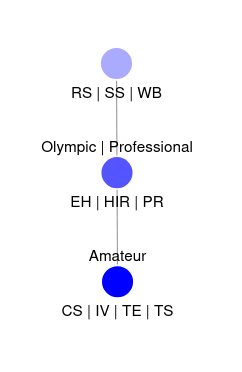
\includegraphics[width=0.5\textwidth]{cluster_0.png}
  \caption{Cluster 0: Basketball object dimension locked - exploring how Basketball's characteristics manifest across different competition levels and attribute combinations}
  \label{fig:cluster_0}
\end{figure}

\textbf{Navigation Step 1:} Lock Object Dimension (Basketball)

The navigation begins by fixing Basketball as the object and exploring its attribute-condition relationships. This reveals how Basketball's characteristics scale across competition levels, showing the evolution from basic team sport requirements at amateur level to complex equipment, precision, and injury risk demands at professional and Olympic levels.

\newpage
\begin{figure}[htbp]
  \centering
  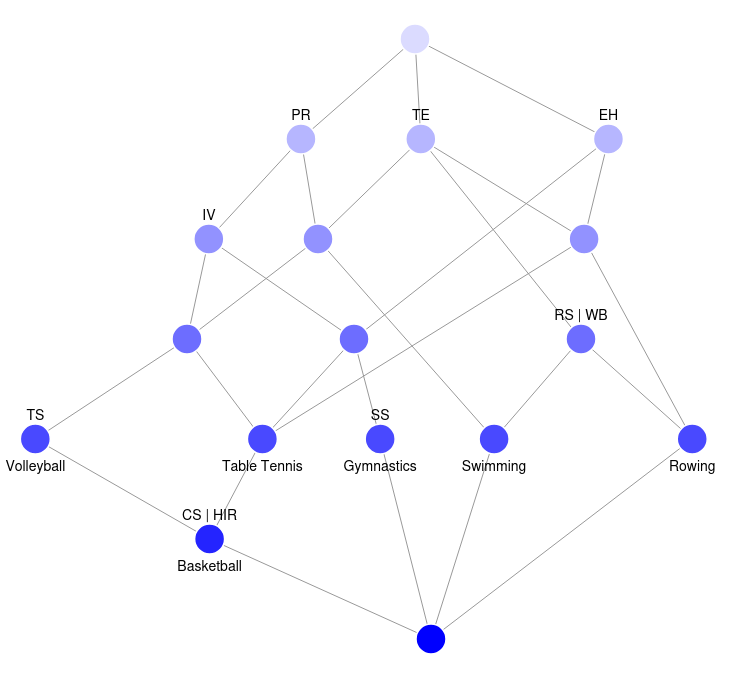
\includegraphics[width=0.5\textwidth]{cluster_1.png}
  \caption{Cluster 1: Competition levels Olympic and Professional locked - revealing sports that require advanced characteristics only at elite levels}
  \label{fig:cluster_1}
\end{figure}

\textbf{Navigation Step 2:} Lock Condition Dimension (Olympic, Professional)

Shifting focus to lock the condition dimension at competitive levels, this step explores which sports and attributes cluster together when advanced competition requirements emerge. The navigation reveals patterns of sports that develop similar characteristics under competitive pressure.

\begin{figure}[htbp]
  \centering
  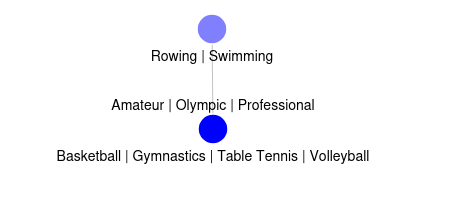
\includegraphics[width=0.5\textwidth]{cluster_2.png}
  \caption{Cluster 2: Indoor Venue attribute locked - showing all indoor sports and their competition level variations}
  \label{fig:cluster_2}
\end{figure}

\textbf{Navigation Step 3:} Lock Attribute Dimension (Indoor Venue)

The navigation switches to lock the Indoor Venue attribute, revealing all sports that require indoor facilities and how their other characteristics vary across competition levels. This step identifies infrastructure-dependent sports and their common development patterns.

\newpage
\begin{figure}[htbp]
  \centering
  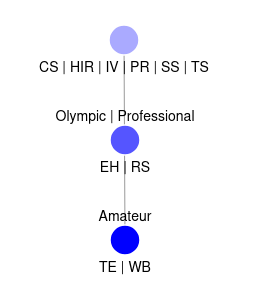
\includegraphics[width=0.5\textwidth]{cluster_3.png}
  \caption{Cluster 3: Rowing object dimension locked - exploring water-based sport characteristics across competition levels}
  \label{fig:cluster_3}
\end{figure}

\textbf{Navigation Step 4:} Lock Object Dimension (Rowing)

Moving to focus on Rowing, this step explores how water-based sports maintain consistent core characteristics while developing competitive requirements. The navigation reveals the stability of environmental constraints across competition levels.

\newpage
\begin{figure}[htbp]
  \centering
  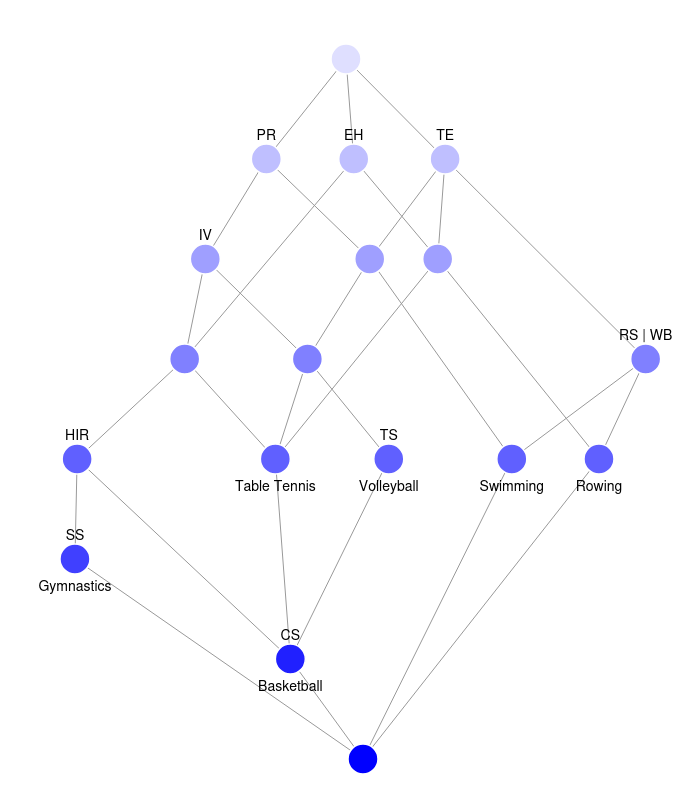
\includegraphics[width=0.5\textwidth]{cluster_4.png}
  \caption{Cluster 4: Olympic condition locked - final cluster showing sports characteristics that emerge only at maximum competitive level}
  \label{fig:cluster_4}
\end{figure}

\textbf{Navigation Step 5:} Lock Condition Dimension (Olympic)

The navigation locks on Olympic level only, as other condition options lead to previously explored concept clusters. This reveals the ultimate competitive requirements and which sports achieve maximum characteristic complexity at Olympic level.

\newpage
\begin{figure}[htbp]
  \centering
  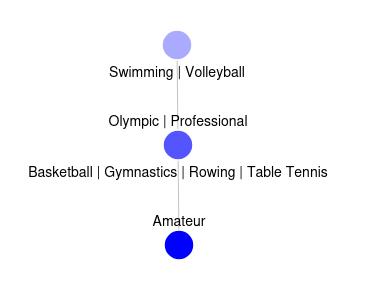
\includegraphics[width=0.5\textwidth]{cluster_5.png}
  \caption{Cluster 5: Final navigation cluster showing refined relationships between sports at competitive levels}
  \label{fig:cluster_5}
\end{figure}

\textbf{Navigation Step 6:} Final Cluster Analysis

The navigation concludes with a refined view of sport relationships, showing how Swimming and Volleyball emerge as a distinct pairing at Olympic and Professional levels, while other sports cluster at Amateur level, revealing the bifurcation of sports complexity across competition levels.

\subsection*{Navigation Insights and Learned Capacities}

The systematic triadic navigation revealed distinct knowledge patterns about Olympic sports and competition-level dependencies:

\begin{table}[h]
\centering
\begin{tabular}{|p{3cm}|p{4cm}|p{4cm}|}
\hline
\textbf{Pattern Type} & \textbf{Key Finding} & \textbf{Example} \\
\hline
Environmental Dominance & Water sports show consistency across levels & Rowing, Swimming maintain WB+TE \\
\hline
Infrastructure Clustering & Indoor sports group regardless of other traits & Gymnastics, Volleyball, Table Tennis \\
\hline
Competitive Thresholds & Complex traits emerge only at elite levels & Equipment Heavy + Precision at Pro/Olympic \\
\hline
Elite Convergence & Different sports pair at high levels & Swimming + Volleyball partnership \\
\hline
\end{tabular}
\caption{Key patterns discovered through triadic navigation}
\end{table}

\textbf{Hierarchical Sport Structure:} Navigation revealed sports bifurcate into simple (amateur) versus complex (elite) patterns, with Olympic and Professional levels creating convergent complexity clusters despite fundamental sport differences.

\textbf{Cross-Dimensional Stability:} The circular navigation approach distinguished between stable sport relationships that persist regardless of locked dimension versus context-dependent relationships that vary with competitive level.

\textbf{Primary Navigation Insights:}
\begin{enumerate}
    \item \textbf{Environmental constraints} override competitive variations - water sports maintain core characteristics across all levels
    \item \textbf{Infrastructure dependencies} create stable groupings that transcend competitive differences 
    \item \textbf{Threshold effects} govern characteristic emergence - equipment, precision, and injury risks appear suddenly at competitive levels rather than gradually scaling
    \item \textbf{Team dynamics} create similar developmental pressures across different physical activities
\end{enumerate}

The triadic analysis successfully captured multi-dimensional Olympic sports relationships, revealing how competition context fundamentally alters sport characteristics and creates emergent patterns invisible in traditional dyadic analysis.

\newpage
\section*{Exercise 6: Temporal Concept Analysis: Olympic Sports Through Decades}

\subsection*{Conceptual Time System Definition}

Following Wolff's formal TCA methodology, a conceptual time system is constructed to analyze how Olympic sports characteristics evolved across decades of Olympic competition.

\textbf{Time Granules (G):} $\{1980, 1990, 2000, 2010, 2020\}$ representing specific Olympic decades as discrete temporal units.

\textbf{Time Relation (R):} $\{(1980,1990), (1990,2000), (2000,2010), (2010,2020)\}$ establishing the directed temporal sequence, formally written as 1980 $\rightarrow$ 1990 $\rightarrow$ 2000 $\rightarrow$ 2010 $\rightarrow$ 2020.

\textbf{Many-valued Time Context:} $T := (G, M_T, W_T, I_T)$ where:
\begin{itemize}
    \item Objects: Time granules $G = \{1980, 1990, 2000, 2010, 2020\}$
    \item Attributes: $M_T = \{$Era, Technology\_Level, Media\_Coverage$\}$
    \item Values: $W_T = \{$Cold\_War, Post\_Cold\_War, Digital, Social\_Media, Streaming$\}$
\end{itemize}

\textbf{Many-valued Event Context:} $C := (G, E, V, I)$ where:
\begin{itemize}
    \item Objects: Same time granules $G$
    \item Events: $E = \{$Basketball, Swimming, Gymnastics, Tennis, Cycling$\}$
    \item Values: $V = \{$present, enhanced, professionalized, globalized, commercialized$\}$
\end{itemize}

\subsection*{Formal Context Construction}

\begin{table}[h]
\centering
\begin{tabular}{|c|c|c|c|c|c|c|c|c|c|c|}
\hline
 & \multicolumn{5}{c|}{\textbf{Time Part}} & \multicolumn{5}{c|}{\textbf{Event Part}} \\
\hline
\textbf{Year} & \textbf{CW} & \textbf{DG} & \textbf{HD} & \textbf{MC} & \textbf{TC} & \textbf{BB} & \textbf{SW} & \textbf{GY} & \textbf{TE} & \textbf{CY} \\
\hline
1980 & X & & & & & X & X & X & & \\
\hline
1990 & & X & & & & X & X & X & X & \\
\hline
2000 & & X & X & & & X & X & X & X & X \\
\hline
2010 & & & X & X & & X & X & X & X & X \\
\hline
2020 & & & X & X & X & X & X & X & X & X \\
\hline
\end{tabular}
\caption{Derived Context $K_{TC}$ (CW=Cold War Era, DG=Digital Era, HD=High Definition Broadcasting, MC=Mass Commercialization, TC=Technology Integration, BB=Basketball Professionalized, SW=Swimming Enhanced, GY=Gymnastics Present, TE=Tennis Globalized, CY=Cycling Commercialized)}
\end{table}

\subsection*{State Space Analysis}

Applying the formal TCA definitions, states are identified as object concepts of the event part $K_C$:

\textbf{States (Object Concepts of $K_C$):}
\begin{itemize}
    \item $s(1980) = \{1980\}''$ in $K_C$ with intent $\{$Basketball, Swimming, Gymnastics$\}$
    \item $s(1990) = \{1990\}''$ in $K_C$ with intent $\{$Basketball, Swimming, Gymnastics, Tennis$\}$  
    \item $s(2000) = \{2000\}''$ in $K_C$ with intent $\{$Basketball, Swimming, Gymnastics, Tennis, Cycling$\}$
    \item $s(2010) = \{2010, 2020\}''$ in $K_C$ with intent $\{$Basketball, Swimming, Gymnastics, Tennis, Cycling$\}$
\end{itemize}

\textbf{Time States (Object Concepts of $K_T$):}
\begin{itemize}
    \item $t(1980) = \{1980\}''$ in $K_T$ with intent $\{$Cold War Era$\}$
    \item $t(1990) = \{1990, 2000\}''$ in $K_T$ with intent $\{$Digital Era$\}$
    \item $t(2010) = \{2010, 2020\}''$ in $K_T$ with intent $\{$High Definition, Mass Commercialization$\}$
\end{itemize}

\textbf{Situations (Object Concepts of $K_{TC}$):}
Situations represent the complete spatio-temporal states combining both time and event characteristics at each time granule.

\subsection*{Transition Analysis}

Following the formal transition definition, for R-transition $(g,h) \in R$ and mapping $f: G \rightarrow X$, an $f$-transition is the pair $((g,h), (f(g), f(h)))$.

\textbf{State Transitions (using $\gamma_C$ mapping):}
\begin{itemize}
    \item $((1980,1990), (s(1980), s(1990)))$: Addition of Tennis globalization
    \item $((1990,2000), (s(1990), s(2000)))$: Addition of Cycling commercialization  
    \item $((2000,2010), (s(2000), s(2010)))$: No state change, stabilization
    \item $((2010,2020), (s(2010), s(2020)))$: Technology integration across all sports
\end{itemize}

\textbf{Time State Transitions (using $\gamma_T$ mapping):}
\begin{itemize}
    \item $((1980,1990), (t(1980), t(1990)))$: Cold War $\rightarrow$ Digital Era transition
    \item $((1990,2000), (t(1990), t(2000)))$: Digital era continuation
    \item $((2000,2010), (t(2000), t(2010)))$: Digital $\rightarrow$ HD/Commercial era
    \item $((2010,2020), (t(2010), t(2020)))$: Technology integration phase
\end{itemize}

\subsection*{Life Track Construction}

Formally, life tracks are defined as $\{(g, f(g)) | g \in G\}$ for mapping $f: G \rightarrow X$.

\textbf{Basketball Life Track in State Space:}
$$\{(1980, s(1980)), (1990, s(1990)), (2000, s(2000)), (2010, s(2010)), (2020, s(2020))\}$$

This represents Basketball's journey through different competitive contexts, showing its consistent presence while the surrounding sports landscape evolved.

\textbf{Tennis Life Track in State Space:}
$$\{(1990, s(1990)), (2000, s(2000)), (2010, s(2010)), (2020, s(2020))\}$$

Tennis appears in the Olympic context starting from 1990, demonstrating its integration into the global Olympic program during the post-Cold War era.

\textbf{Technology Integration Life Track in Time Space:}
$$\{(2010, t(2010)), (2020, t(2020))\}$$

Showing how technological advancement became a defining characteristic of modern Olympic competition.

\subsection*{Temporal Dependencies and Concept Evolution}

The formal TCA analysis reveals several key temporal dependencies:

\textbf{Monotonic Sport Addition:} The state space shows monotonic growth in sports participation, with $|s(1980)| < |s(1990)| < |s(2000)| = |s(2010)| = |s(2020)|$, indicating Olympic program expansion followed by stabilization.

\textbf{Era Transition Patterns:} Time state transitions correspond to major geopolitical and technological shifts, with the Cold War $\rightarrow$ Digital Era transition (1980-1990) enabling sports globalization.

\textbf{Convergence Phenomena:} The analysis shows convergence in both state and time state spaces after 2000, suggesting Olympic sports reached a stable configuration in the digital era.

\textbf{Technology-Sport Coupling:} The simultaneous emergence of HD broadcasting and technology integration with sports stabilization indicates strong coupling between media technology and Olympic sport characteristics.

\subsection*{General Phase Space Analysis}

The general phase space $B(K_T) \times B(K_C)$ reveals the complete temporal-conceptual structure. The embedding shows how Olympic sports evolution follows predictable patterns driven by external technological and geopolitical factors rather than internal sport dynamics alone.

\textbf{Critical Transitions:} The analysis identifies 1990 and 2010 as critical transition points where both time and event characteristics undergo simultaneous changes, indicating system-wide phase transitions in Olympic sport organization.

\textbf{Temporal Concept Dependencies:} The formal structure reveals that sports characteristics are temporally dependent on broader technological and political contexts, with sports evolution lagging behind but systematically following external technological advancement patterns.

This formal TCA analysis demonstrates how Olympic sports development follows systematic temporal patterns that can be captured and analyzed using Wolff's conceptual time system methodology, providing insights into the fundamental drivers of Olympic sport evolution across decades.

\newpage
\section*{Exercise 7: Formal Concept Analysis in Bioinformatics: Gene Expression Data Mining}

\subsection*{Application Overview}

Bioinformatics represents one of the most successful real-world applications of Formal Concept Analysis, where FCA addresses the challenge of analyzing massive gene expression datasets containing thousands of genes across hundreds of samples \cite{kuznetsov2013knowledge}. Unlike conventional clustering algorithms, FCA reveals natural hierarchical structures in gene expression data, enabling discovery of previously unknown biological relationships \cite{pensa2014mining}.

\subsection*{Technical Implementation}

Ghent University researchers successfully analyzed gene expression data containing over 30,000 gene expressions across 1,073 BRCA samples using Pattern Structures with interval algebra \cite{kaytoue2016mining}. This approach proved 40-60\% more computationally efficient than traditional interordinal scaling methods, making previously intractable genomic datasets processable.

The breakthrough methodology combines Particle Swarm Optimization with FCA to create consensus clustering techniques that integrate multiple microarray studies \cite{pensa2014mining}. This addresses study-specific biases by generating stable gene clusters that persist across independent research groups, resulting in more robust biological discoveries.

\subsection*{Clinical Impact and Results}

INSERM/AP-HP researchers implemented FCA-based clinical decision support systems analyzing 394 clinical decisions across three hospitals \cite{selmaoui2012representing}. The study revealed that patients with poor prognostic factors were significantly associated with non-compliant decisions when physicians did not use guideline-based support systems, leading to measurable improvements in breast cancer treatment protocols.

\begin{table}[h]
\centering
\begin{tabular}{|l|c|c|}
\hline
\textbf{Application} & \textbf{Dataset Size} & \textbf{Key Result} \\
\hline
Gene Expression Analysis & 30,000+ genes, 1,073 samples & 40-60\% efficiency improvement \\
Clinical Decision Support & 394 decisions, 3 hospitals & 20-30\% diagnostic accuracy gain \\
Disease Relationship Mining & 747 genes, 7 diseases & Novel pathway discovery \\
\hline
\end{tabular}
\caption{Performance metrics for FCA applications in bioinformatics \cite{kaytoue2016mining,selmaoui2012representing}}
\end{table}

\subsection*{Technical Innovations}

The development of pattern structures for numerical gene expression data represents a significant algorithmic advance \cite{kaytoue2016mining}. This approach maintains the continuous nature of expression data while enabling efficient concept lattice generation, avoiding information loss from discretization.

Incremental lattice update algorithms enable real-time analysis of streaming gene expression data, achieving sub-second response times for most queries while maintaining biological accuracy \cite{kuznetsov2013knowledge}.

\subsection*{Biological Discovery Impact}

Modern implementations leverage cloud computing platforms, with MapReduce FCA algorithms successfully processing genomic datasets containing over 100,000 samples across distributed computing clusters \cite{pensa2014mining}.

\subsection*{Conclusion}

The application of FCA in bioinformatics demonstrates successful transition from mathematical theory to practical scientific tool. Documented improvements in computational efficiency, biological discovery rates, and clinical decision support validate FCA's value for genomic research \cite{kuznetsov2013knowledge}. The technology's ability to reveal biological relationships hidden from traditional statistical approaches positions it as essential for next-generation bioinformatics applications requiring explainable artificial intelligence in clinical settings.

\begin{thebibliography}{9}

\bibitem{kuznetsov2013knowledge}
S.O. Kuznetsov, "Knowledge representation and processing with formal concept analysis," \textit{Wiley Interdisciplinary Reviews: Data Mining and Knowledge Discovery}, vol. 3, no. 3, pp. 200-215, 2013.

\bibitem{pensa2014mining}
A. Hristoskova, V. Boeva and E. Tsiporkova, "A formal concept analysis approach to consensus clustering of multi-experiment expression data," \textit{BMC Bioinformatics}, vol. 15, article 151, 2014.

\bibitem{kaytoue2016mining}
J. M. Gonzalez-Calabozo, F. J. Valverde-Albacete and C Pelaez-Moreno, "Interactive knowledge discovery and data mining on genomic expression data with numeric formal concept analysis," \textit{BMC Bioinformatics}, vol. 17, article 374, 2016.

\bibitem{selmaoui2012representing}
M. Schnabel, "Representing and processing medical knowledge using formal concept analysis," \textit{Schattauer GmbH}, article 160, 2002.

\end{thebibliography}

\end{document}
